%!TEX program = xelatex
% 完整编译: xelatex -> biber/bibtex -> xelatex -> xelatex
\documentclass[lang=cn,11pt,a4paper]{elegantpaper}

\title{词法分析程序的设计与实现}
\author{杨晨 \\学号2021212171}
\institute{北京邮电大学 计算机学院}

% \version{0.10}
\date{2023年10月1日}

% 本文档命令
\usepackage{array}
\usepackage{xcolor}
\newcommand{\ccr}[1]{\makecell{{\color{#1}\rule{1cm}{1cm}}}}

% 设置代码样式
\lstset{
    language=C++, % 设置代码语言为C++
    basicstyle=\ttfamily, % 设置基本字体样式为等宽字体
    backgroundcolor=\color{gray!10}, % 设置代码块背景颜色为白色
    commentstyle=\color{green!60!black}, % 设置注释颜色
    keywordstyle=\color{blue}, % 设置关键字颜色
    stringstyle=\color{orange}, % 设置字符串颜色
    showstringspaces=false, % 不显示字符串中的空格符
    breaklines=true, % 自动断行
    numbers=left, % 行号显示在左侧
    numberstyle=\small\color{gray}, % 设置行号样式
    frame=single, % 绘制代码框
    rulecolor=\color{black}, % 设置代码框颜色
    captionpos=b, % 设置标题位置为底部
    tabsize=4, % 设置制表符宽度
    keywordstyle=[1]\color{blue}, % 设置关键字样式
    keywordstyle=[2]\color{purple}, % 设置扩展关键字样式
    keywordstyle=[3]\color{teal}, % 设置内置类型样式
    keywordstyle=[4]\color{magenta}, % 设置注解样式
    keywordstyle=[5]\color{orange}, % 设置预处理指令样式
    keywordstyle=[6]\color{cyan!60!black}, % 设置其他关键字样式
    keywordstyle=[7]\color{violet}, % 设置特殊关键字样式
}

\begin{document}



\maketitle
\tableofcontents

\section{概述}

\subsection{实验内容}

\begin{enumerate}
    \item 选定源语言,c语言
    \item 可以识别出用源语言编写的源程序中的每个单词符号,并以记号的形式输出每个单词符号。
    \item 可以识别并跳过源程序中的注释。
    \item 可以统计源程序中的语句行数、各类单词的个数、以及字符总数,并输出统计结果。
    \item 检查源程序中存在的词法错误,并报告错误所在的位置。
    \item 对源程序中出现的错误进行适当的恢复,使词法分析可以继续进行,对源程序进行一次扫描,即可检查并报告源程序中存在的所有词法错误。
\end{enumerate}

\subsection{开发环境}

\begin{itemize}
    \item Windows10
    \item Visual Studio Code
\end{itemize}

\section{程序的功能模块划分}

\subsection{识别数值}

\begin{figure}[!htb]
    \centering
    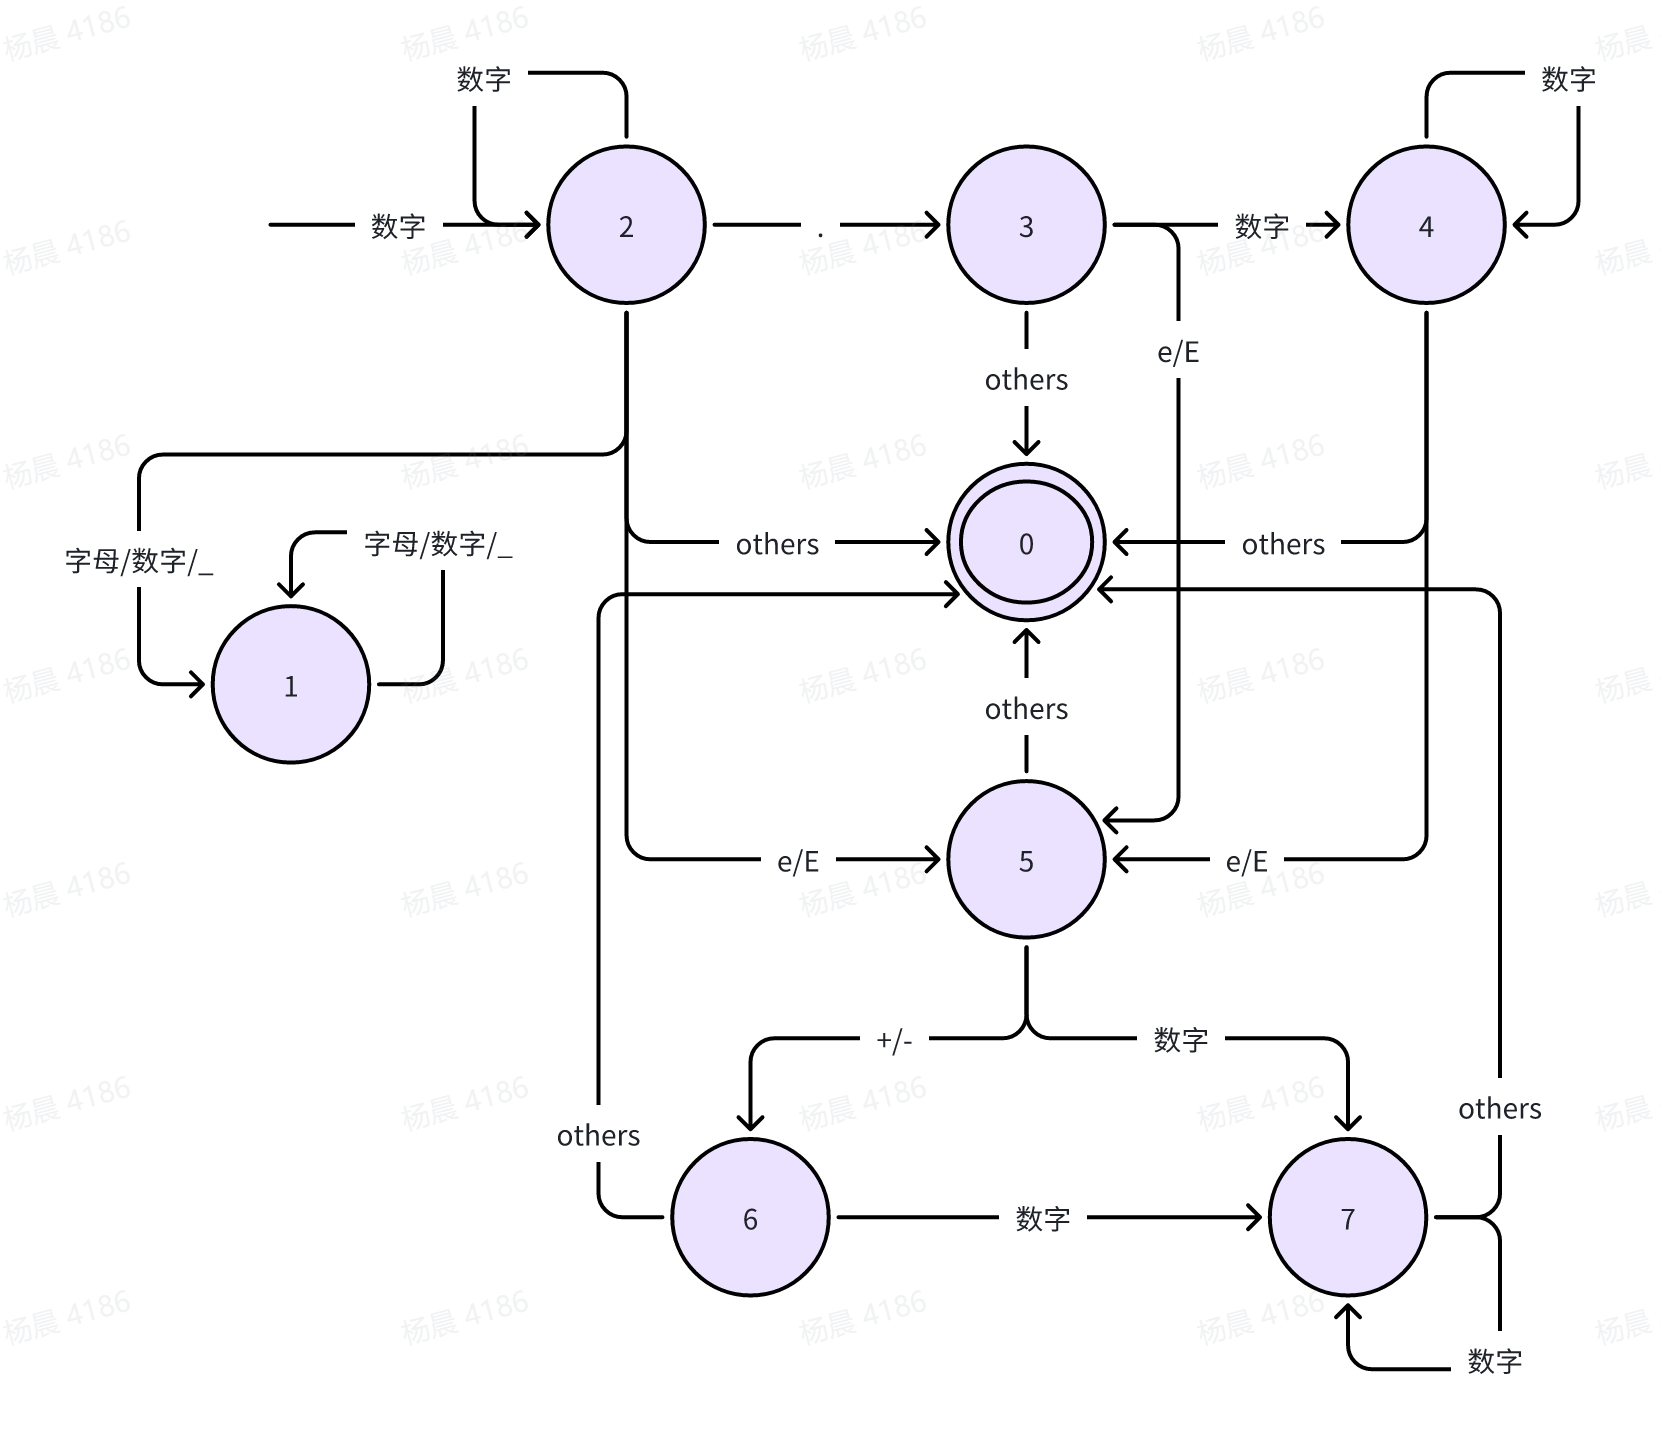
\includegraphics[width=0.9\textwidth]{image/Numerical.png}
    \caption{识别Numerical的自动机}
\end{figure}

在代码中,我参考了课上的PPT中关于数值识别的自动机设计,并根据您的需求进行了修改。这个自动机用于识别数值常量,并根据常规的数值表示规则确定常量的类型。

状态2是数值常量的起始状态,状态3表示遇到了小数点,状态4表示小数点后的数字,状态5表示遇到了指数符号,状态6表示指数符号后的正负号,状态7表示指数后的数字。

该自动机的工作过程如下:
\begin{itemize}
    \item 初始状态为状态2,开始处理数值常量。
    \item 通过循环遍历输入字符,并根据当前状态和输入字符执行相应的操作。
    \item 在状态2中,如果遇到数字,则保持状态2并继续前进,如果遇到小数点,则转移到状态3,如果遇到指数符号,则转移到状态5,如果遇到不是e(E)的字母,则将token的类型设置为\lstinline{"Error"},并记录错误信息。
    \item 在状态3中,如果遇到数字,则转移到状态4,表示遇到小数点后的数字部分。如果遇到指数符号,则转移到状态5,遇到其他字符(非\lstinline{;}),则将token的类型设置为\lstinline{"Error"},并记录错误信息。
    \item 在状态4中,如果遇到数字,则保持状态4并继续前进,如果遇到指数符号,则转移到状态5,如果遇到其他字符,则将token的类型设置为\lstinline{"Error"},并记录错误信息。
    \item 在状态5中,如果遇到数字,则转移到状态7,表示遇到指数后的数字部分。如果遇到正负号,则转移到状态6,表示遇到指数后的正负号。如果遇到其他字符,则将token的类型设置为\lstinline{"Error"},并记录错误信息。
    \item 在状态6中,如果遇到数字,则转移到状态7,表示遇到指数后的数字部分。如果遇到其他字符,则将token的类型设置为\lstinline{"Error"},并记录错误信息。
    \item 在状态7中,如果遇到数字,则保持状态7并继续前进,如果遇到其他字符,则将token的类型设置为\lstinline{"Error"},并记录错误信息。
    \item 当自动机状态变为0时,表示数值常量识别结束。
\end{itemize}

\subsection{识别单字符常量}

\begin{figure}[!htb]
    \centering
    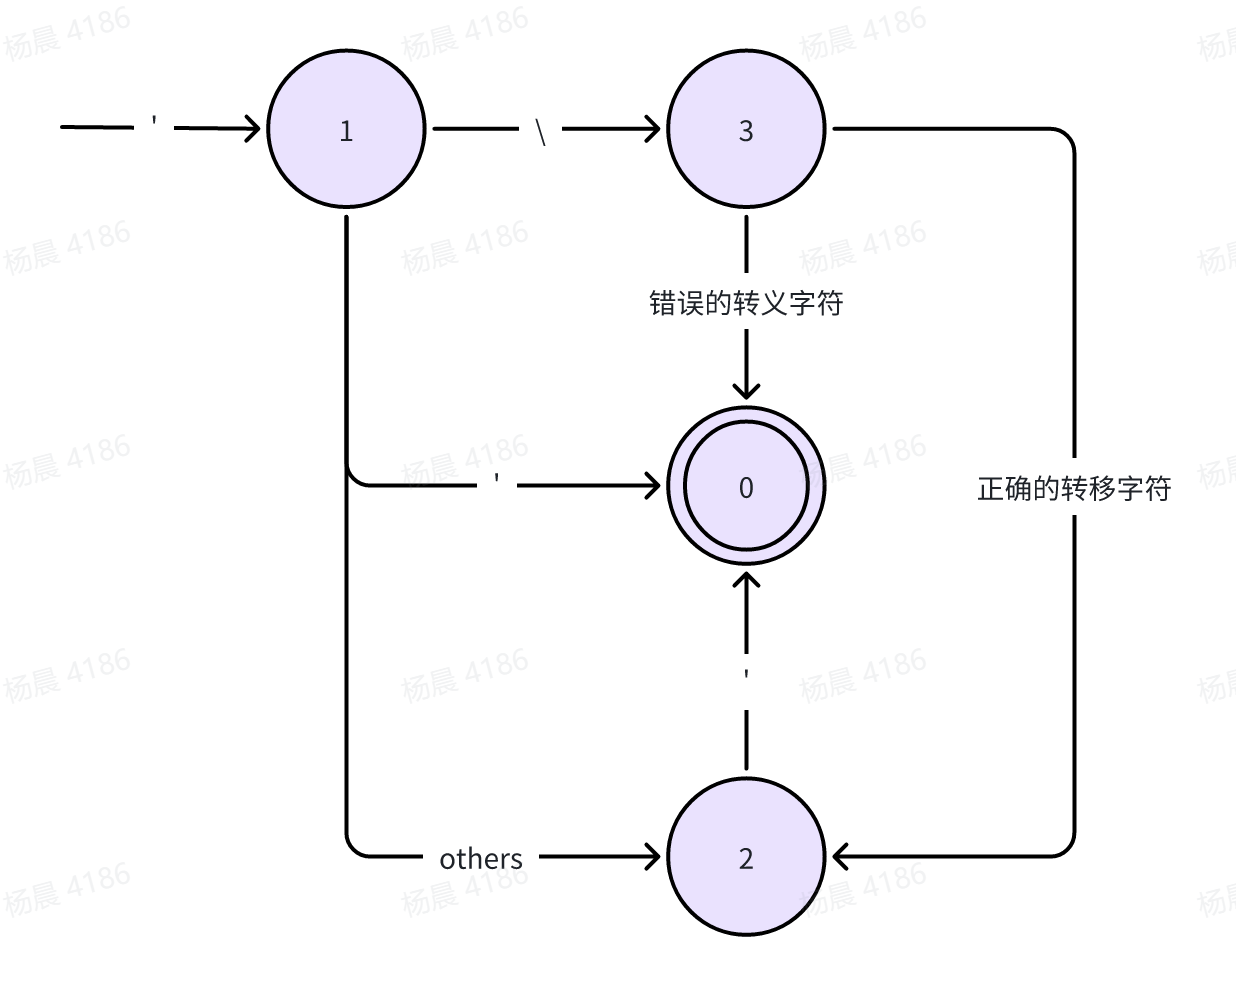
\includegraphics[width=0.9\textwidth]{image/Char.png}
    \caption{识别CharConstant的自动机}
\end{figure}

这个自动机实现了一个自动机来识别字符常量。自动机的初始状态为1,表示开始处理字符常量。

该自动机的工作过程如下:
\begin{itemize}
    \item 在状态1中,首先检查下一个字符。如果下一个字符是反斜杠(\char`\\),则表示遇到了转义字符,进入状态3。如果下一个字符是单引号('),则表示遇到了空字符,进入状态0。否则,进入状态2,表示遇到了普通字符。
    \item 在状态2中,继续读取下一个字符。如果下一个字符是单引号('),则表示字符常量结束,进入状态0。否则,表示遇到了多字符字符常量或者遇到了未闭合的单引号('),将token的类型设置为"\lstinline{"Error"},并记录错误信息。
    \item 在状态3中,继续读取下一个字符。如果下一个字符是合法的转义字符(例如:a、b、f、n、r、t、v、\char`\\、'、"、?),则进入状态2,表示转义字符合法。否则,表示遇到了非法的转义字符,将token的类型设置为\lstinline{"Error"},并记录错误信息。
    \item 当自动机状态变为0时,表示字符常量识别结束。
\end{itemize}

\subsection{识别字符串常量}

\begin{figure}[!htb]
    \centering
    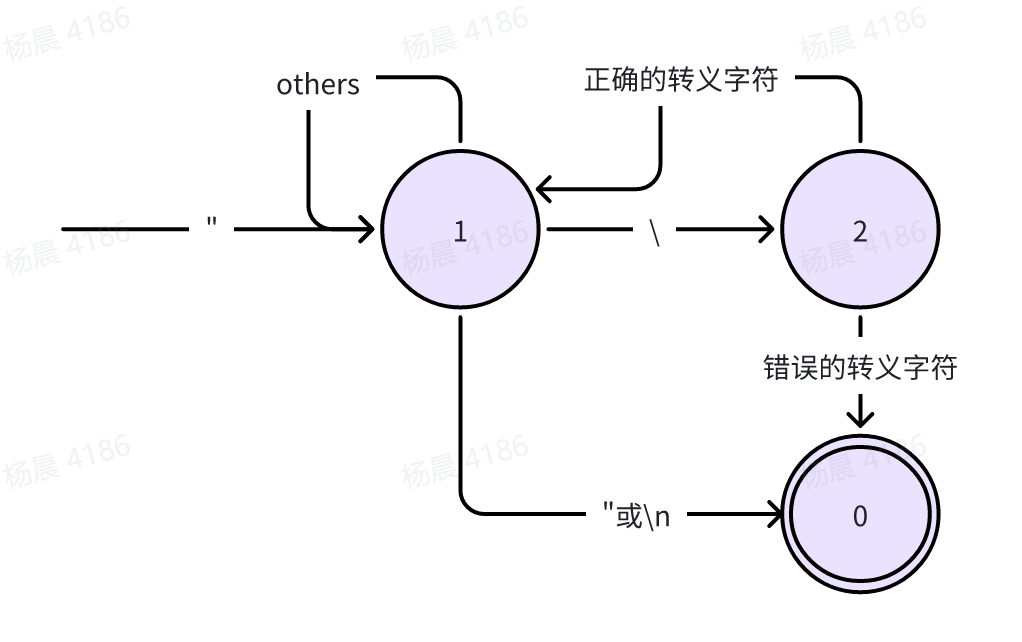
\includegraphics[width=0.9\textwidth]{image/String.png}
    \caption{识别StringLiteral的自动机}
\end{figure}

这段代码实现了一个自动机来识别字符串字面串。自动机的初始状态为1,表示开始处理字符常量。

自动机的工作原理如下:
\begin{itemize}
    \item 在状态1中,首先检查下一个字符。如果下一个字符是反斜杠(\char`\\),则表示遇到了转义字符,进入状态3。如果下一个字符是单引号('),则表示遇到了空字符,进入状态0。否则,进入状态2,表示遇到了普通字符。
    \item 在状态2中,继续读取下一个字符。如果下一个字符是单引号('),则表示字符常量结束,进入状态0。否则,表示遇到了多字符字符常量,将token的类型设置为\lstinline{"Error"},并记录错误信息。
    \item 在状态3中,继续读取下一个字符。如果下一个字符是合法的转义字符(例如:a、b、f、n、r、t、v、\char`\\、'、"、?),则进入状态2,表示转义字符合法。否则,表示遇到了非法的转义字符,将token的类型设置为\lstinline{"Error"},并记录错误信息。
    \item 当自动机状态变为0时,表示字符常量识别结束,根据buffer中的内容设置token的值。
\end{itemize}

通过这个自动机,您可以识别并解析输入中的字符常量,并根据识别结果设置相应的token类型和值。当遇到转义字符时,自动机能够正确处理合法的转义字符,同时也能检测到非法的转义字符并报告错误。

\subsection{各类标点符号}

\begin{lstlisting}
if (!isWhitespace(c))
{
    Token token("Punctuator", countLine, countColumn, "");
    eatChar();
    bool has_error = false;
    bool is_comment = false;
    switch (c) // 标点符号的特殊处理
    {
    case '.': // 识别.或...
        c = peekChar();
        if (c == '.')
        {
            eatChar();
            if ((c = peekChar()) == '.') // 识别...
            {
                eatChar();
            }
            else // 识别错误的省略号
            {
                has_error = true;
                token.setType("Error");
            }
        }
        break;
    case '>': // >或>=或>>或>>=
        c = peekChar();
        if (c == '>') // >>或>>=
        {
            eatChar();
            c = peekChar();
            if (c == '=') // >>=
            {
                eatChar();
            }
        }
        else if (c == '=') // >=
            eatChar();
        break;
    case '<': // <或<=或<<或<<=
        c = peekChar();
        if (c == '<') // <<或<<=
        {
            eatChar();
            if ((c = peekChar()) == '=') // <<=
            {
                eatChar();
            }
        }
        else if (c == '=') // <=
            eatChar();
        break;
    case '+': // +或++或+=
        c = peekChar();
        if (c == '=' || c == '+')
            eatChar();
        break;
    case '-': // -或--或-=或->
        c = peekChar();
        if (c == '=' || c == '-' || c == '>')
            eatChar();
        break;
    case '&': // &或&&或&=
        c = peekChar();
        if (c == '=' || c == '&')
            eatChar();
        break;
    case '|': // |或||或|=
        c = peekChar();
        if (c == '=' || c == '|')
            eatChar();
        break;
    case '*':
    case '%':
    case '^':
    case '=':
    case '!':
        c = peekChar();
        if (c == '=') // *=或%=或^=或==或!=
            eatChar();
        break;
    case ';':
    case '{':
    case '}':
    case ',':
    case ':':
    case '(':
    case ')':
    case '[':
    case ']':
    case '~':
    case '?':
        break; // 单字符标点符号
    case '#':  // 预处理指令,如#include
        is_comment = true; // 预处理指令不输出
        do
        {
            c = eatChar();
        } while (c != '\n'); // 跳过一行
        break;
    case '/': // /或/=或/*或//
        c = peekChar();
        if (c == '*' || c == '/') // 注释
        {
            ... // 在下一个subsection分析
        }
        else if (c == '=') // /=
            eatChar();
        break;
    default: // 未知字符
        has_error = true;
        token.setType("Error");
        token.setError("unexpected character");
        count_Error++;
        token.setValue(buffer);
        break;
    }
    res &= !has_error; // 词法分析是否成功, 有错误返回false
    if (!is_comment)   // 注释不输出
    {
        if (token.getType() == "Punctuator")
        {
            count_Punctuator++;
        }
        token.setValue(buffer);
        std::cout << token << std::endl;
    }
    else if (has_error) // 有错误输出错误信息
    {
        std::cout << token << std::endl;
    }
}
else
{
    eatChar();
}
\end{lstlisting}

该代码片段对字符流进行词法分析,并识别各种标点符号。其大体流程如下

\begin{itemize}
    \item 代码片段首先检查当前字符 c 是否为空白字符。如果不是空白字符,分析过程继续。
    \item 创建一个 Token 对象,将其类型设为 \lstinline"Punctuator",并初始化行号和列号。
    \item 调用 \lstinline{eatChar()} 函数来消耗当前字符,并移动到流中的下一个字符。
    \item 代码使用 switch 语句来处理不同的标点符号和特殊情况。
    \item 对于每个标点符号,代码检查下一个字符(\lstinline{peekChar()}),并根据观察到的模式执行特定的操作。
    \item 如果在分析标点符号过程中遇到任何错误,将将变量 \lstinline{has_error} 设为 \lstinline{true},并将 Token 对象的类型设为 \lstinline{"Error"}。错误消息也相应地设置。
    \item 代码跟踪遇到的错误数量(\lstinline{count_Error})和识别的标点符号数量(\lstinline{count_Punctuator})。
    \item 如果分析的字符是预处理指令的一部分(例如以 \lstinline{'#'} 开头的行),则视为注释并跳过直到行末。
    \item 如果字符不是注释,则将 Token 对象的值设置为处理后的缓冲区,并将其输出到控制台。
    \item 如果字符是注释,但同时存在错误,则将错误消息输出到控制台。
    \item 如果字符是空白字符,则使用 \lstinline{eatChar()} 函数将其消耗掉。
\end{itemize}

上述代码片段展示了词法分析过程中对字符流中标点符号进行识别和处理的一部分。使用 switch 语句来处理不同的标点符号模式和特殊情况。代码跟踪分析过程中遇到的错误,并相应地输出识别的标记和错误消息。

\subsection{识别注释}

\begin{figure}[!htb]
    \centering
    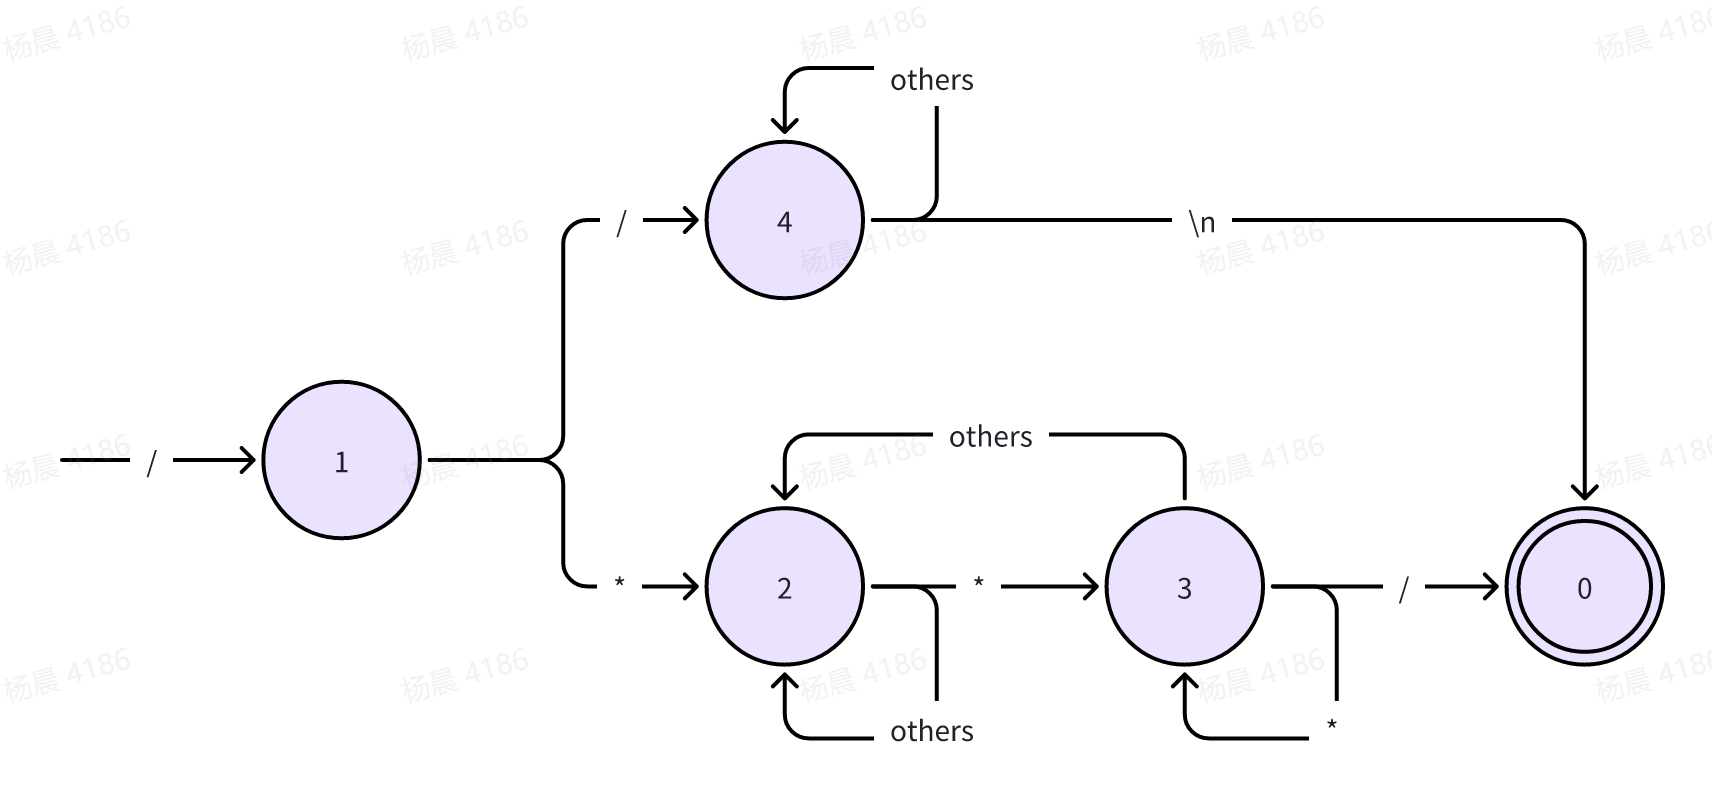
\includegraphics[width=0.9\textwidth]{image/Comment.png}
    \caption{识别Comment的自动机}
\end{figure}

该自动机是用于识别和处理注释的。它基于状态转换的原理,根据输入字符的不同,切换自动机的状态,以便正确识别和处理不同类型的注释。

自动机的工作原理如下:
\begin{itemize}
    \item 当遇到字符 '/' 时,首先检查下一个字符。如果下一个字符是 '*' 或 '/',则表示遇到了注释开始标记,进入注释处理状态。如果下一个字符是 '*',则进入状态2,表示遇到了多行注释。如果下一个字符是 '/',则进入状态4,表示遇到了单行注释。
    \item 状态2表示多行注释中的内容。如果下一个字符是 '*',则进入状态3,表示可能是注释的结束。否则,继续保持在状态2,表示注释内容继续。
    \item 状态3用于判断是否遇到了多行注释的结束。如果下一个字符是 '*',继续保持在状态3。如果下一个字符是 '/',则表示多行注释结束,进入状态0,注释处理结束。否则,说明还处于多行注释中,回到状态2。
    \item 状态4表示单行注释中的内容。如果下一个字符是 '\char`\\n',则表示单行注释结束,进入状态0,注释处理结束。否则,继续保持在状态4,表示注释内容继续。
    \item 状态0表示注释处理结束。
\end{itemize}

通过上述自动机,可以识别和处理不同类型的注释,包括多行注释和单行注释。自动机能够正确识别注释的开始和结束,并在注释处理结束后返回状态0。

\subsection{词法分析总框架}

\begin{figure}[!htb]
    \centering
    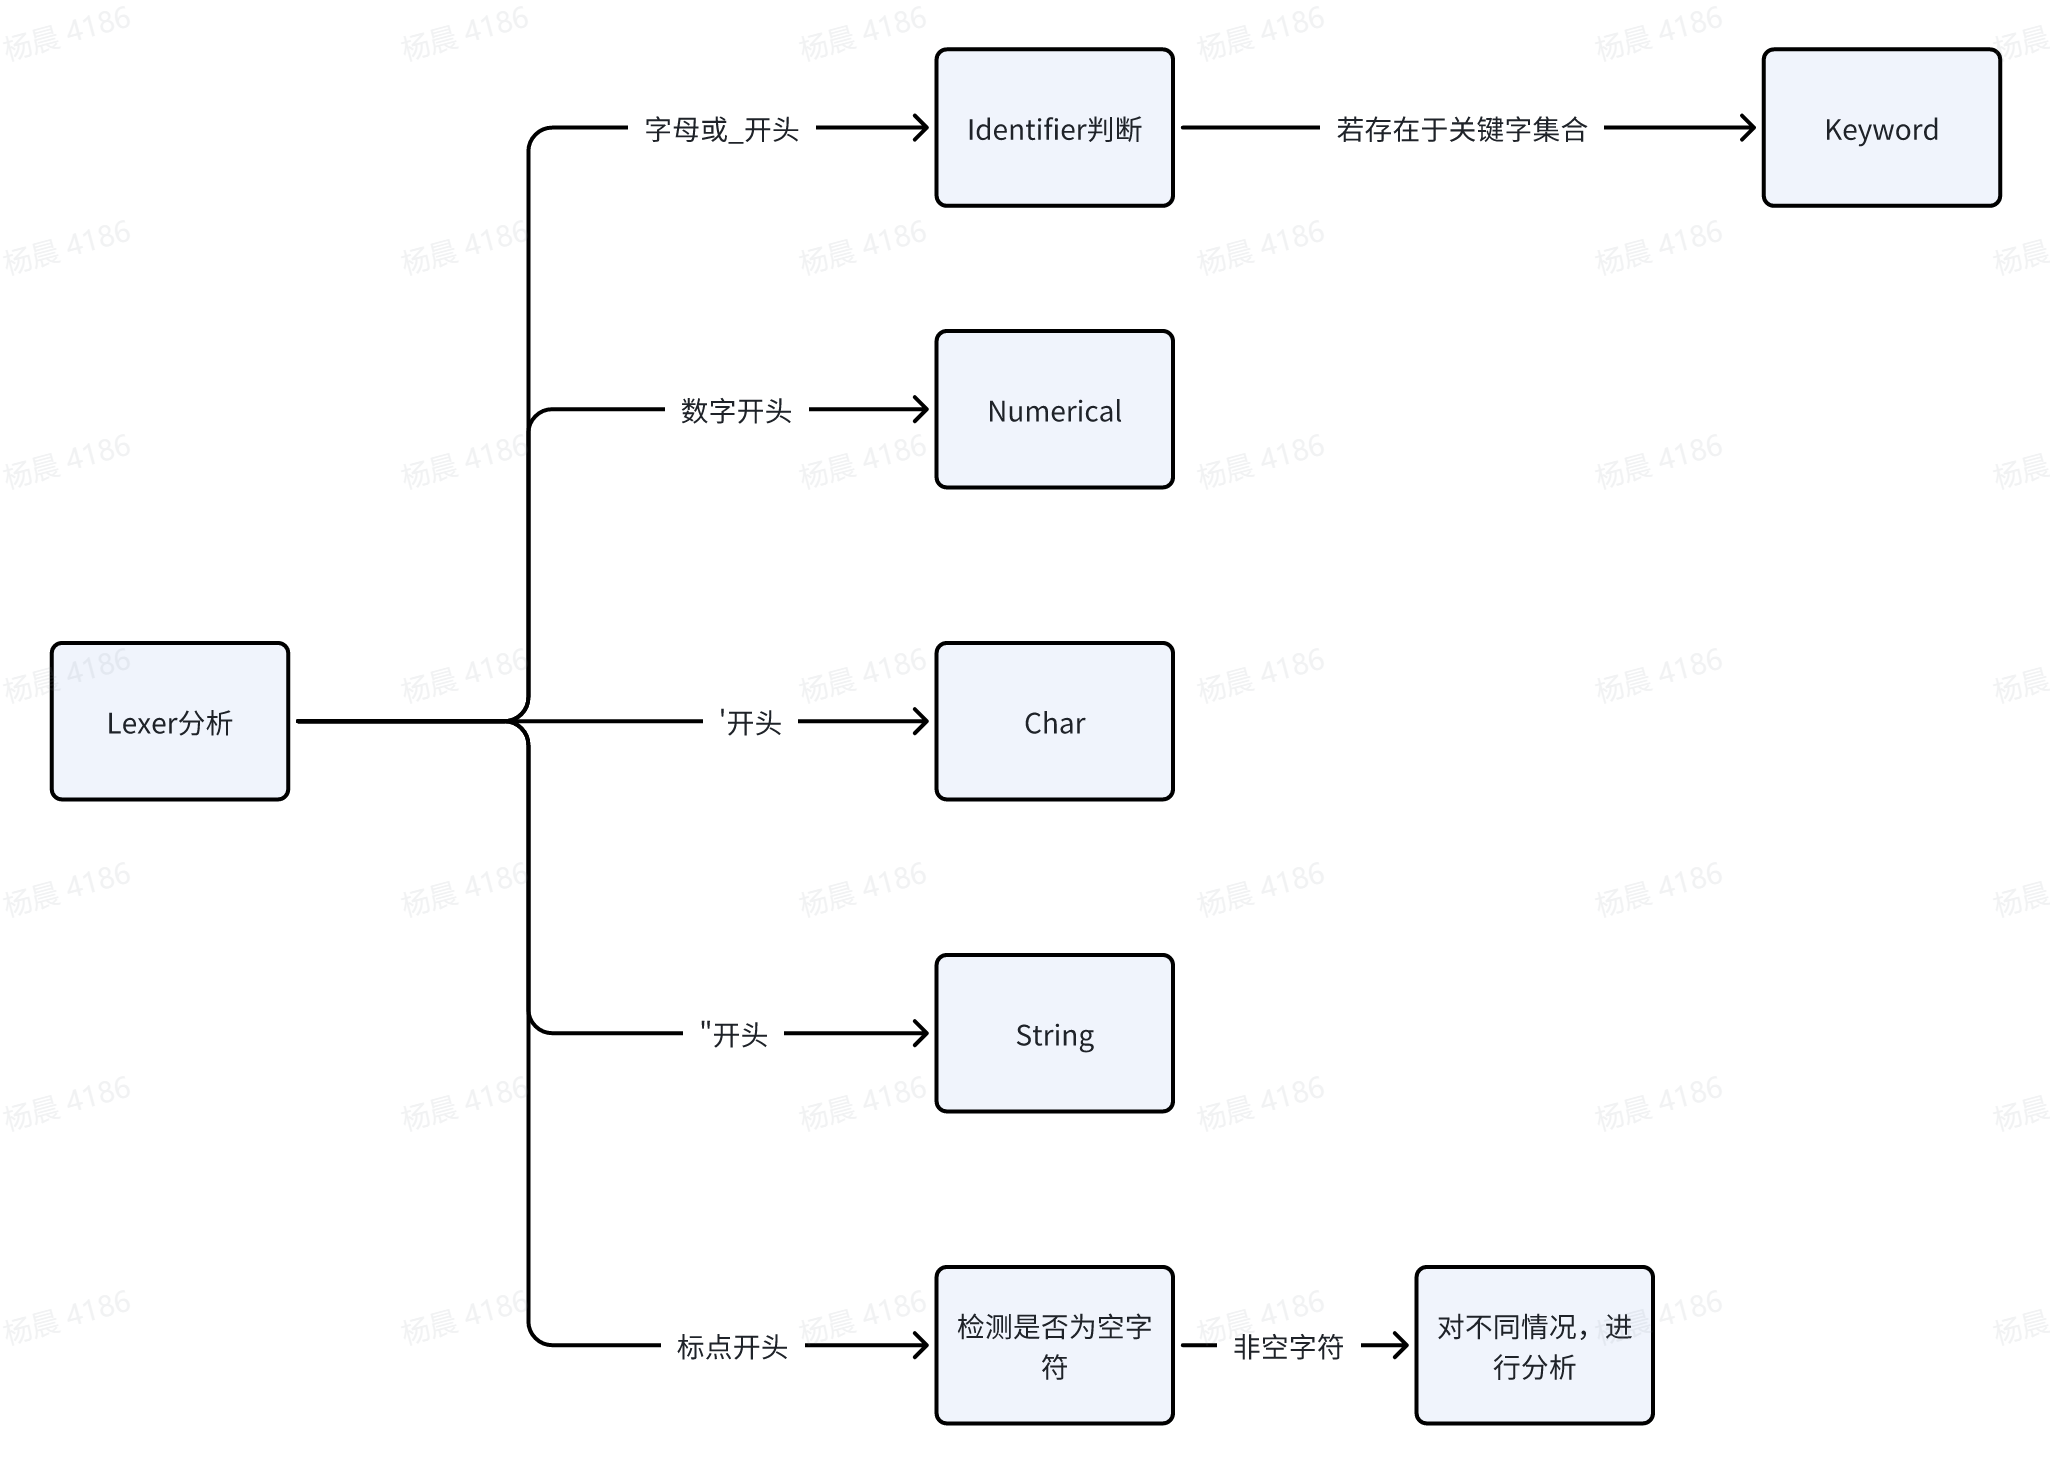
\includegraphics[width=0.9\textwidth]{image/Framework.png}
    \caption{词法分析流程}
\end{figure}

它从输入流中读取字符,直到文件结束或输入缓冲区中没有更多的字符为止。对于每个字符,它检查它是否是字母、数字、单引号、双引号或标点符号。

如果字符是字母,则假设它是标识符或关键字。它创建一个类型为 \lstinline{"Identifier"} 的 Token 对象,并调用\lstinline{getNextIdentifier()}函数从输入流中读取标识符的其余部分。如果标识符与预定义的关键字之一匹配,则词法分析器将标记的类型设置为 "Keyword",并增加一个计数器以记录找到的关键字数。

如果字符是数字,则假设它是数字常量。它创建一个类型为 \lstinline{"Numerical_Constant"} 的 Token 对象,并调用 
\lstinline{getNextNumerical()} 函数从输入流中读取数字常量的其余部分。

如果字符是单引号,则会假设它是字符常量。它创建一个类型为 \lstinline{"Char_Constant"} 的 Token 对象,并调用 \lstinline{getCharConstant()} 函数从输入流中读取字符常量的其余部分。

如果字符是双引号,则会假设它是字符串字面量。它创建一个类型为 \lstinline{"String_Literal"} 的 Token 对象,并调用 \lstinline{getStringLiteral()} 函数从输入流中读取字符串字面量的其余部分。

如果字符是标点符号,则会创建一个类型为 \lstinline{"Punctuator"} 的 Token 对象,并调用 \lstinline{eatChar()} 函数从输入流中消耗字符。然后,它检查标点符号是否是特殊情况,例如点、大于号、小于号、加号、减号、和号、竖线、星号、百分号、脱字符、等号或感叹号。对于每个特殊情况,词法分析器执行适当的操作,例如从输入流中消耗额外的字符或如果遇到意外字符则将标记的类型设置为 \lstinline{"Error"}。

词法分析器还处理注释和预处理指令。如果词法分析器遇到井号,它会假设它是预处理指令,例如 \lstinline{#include}。它消耗该行的其余部分并忽略该指令。如果词法分析器遇到正斜杠,它会检查它是否是注释,单行注释或多行注释。如果它是注释,则词法分析器消耗注释的其余部分并忽略它。

\section{使用说明}

在main.cpp中,可以指定源代码文件的路径
\begin{lstlisting}[numbers = none]
    Lexer lexer("../test/test1.c");
\end{lstlisting}
运行main.cpp后,将会输出词法分析的结果,如下
\begin{figure}[!htb]
    \centering
    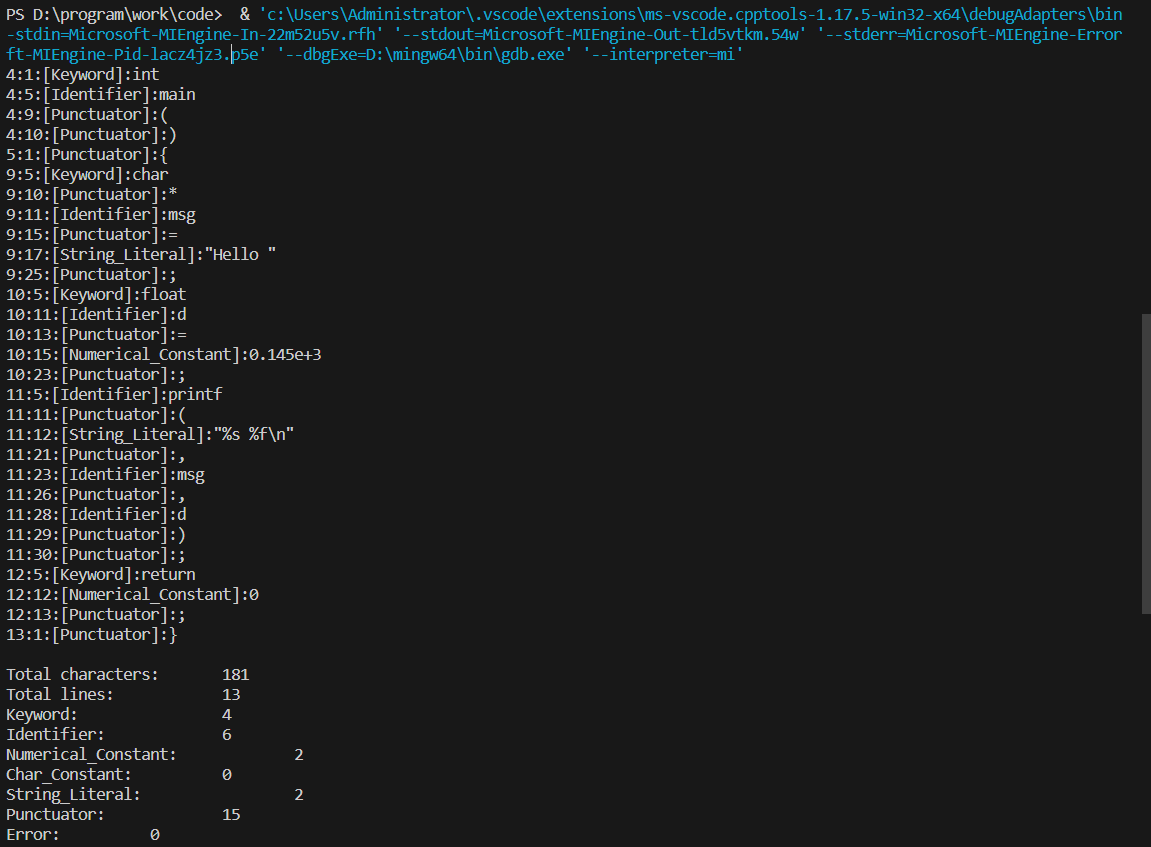
\includegraphics[width=0.9\textwidth]{image/TestResult.png}
    \caption{程序运行效果}
\end{figure}

\clearpage

\section{测试}

\subsection{测试集1}
该测试集用于测试程序在没有词法错误时,是否能正常运行。

\subsubsection{输入的源代码}

\begin{lstlisting}
// Line comment *///*/
#include <stdio.h>

int main()
{
    /*
     * Block comment *
     */
    char *msg = "Hello ";
    char ch = 'w';
    float f = 0.145e+3;
    double d = 3.e3;
    float f2 = 0.145e-3;
    double d2 = 3.;
    int integer = 864;
    long long int longint = 1234567890123456789;
    printf("%s %f\n", msg, d);
    printf("%c\t%d\n", ch, integer);
    printf("%lld\v", longint);
    return 0;
}
\end{lstlisting}

\subsubsection{输出结果}

\begin{lstlisting}[numbers = none, keywordstyle=\color{black},stringstyle=\color{black}]
4:1:[Keyword]:int
4:5:[Identifier]:main
4:9:[Punctuator]:(
4:10:[Punctuator]:)
5:1:[Punctuator]:{
9:5:[Keyword]:char
9:10:[Punctuator]:*
9:11:[Identifier]:msg
9:15:[Punctuator]:=
9:17:[String_Literal]:"Hello "
9:25:[Punctuator]:;
10:5:[Keyword]:char
10:10:[Identifier]:ch
10:13:[Punctuator]:=
10:15:[Char_Constant]:'w'
10:18:[Punctuator]:;
11:5:[Keyword]:float
11:11:[Identifier]:f
11:13:[Punctuator]:=
11:15:[Numerical_Constant]:0.145e+3
11:23:[Punctuator]:;
12:5:[Keyword]:double
12:12:[Identifier]:d
12:14:[Punctuator]:=
12:16:[Numerical_Constant]:3.e3
12:20:[Punctuator]:;
13:5:[Keyword]:float
13:11:[Identifier]:f2
13:14:[Punctuator]:=
13:16:[Numerical_Constant]:0.145e-3
13:24:[Punctuator]:;
14:5:[Keyword]:double
14:12:[Identifier]:d2
14:15:[Punctuator]:=
14:17:[Numerical_Constant]:3.
14:19:[Punctuator]:;
15:5:[Keyword]:int
15:9:[Identifier]:integer
15:17:[Punctuator]:=
15:19:[Numerical_Constant]:864
15:22:[Punctuator]:;
16:5:[Keyword]:long
16:10:[Keyword]:long
16:15:[Keyword]:int
16:19:[Identifier]:longint
16:27:[Punctuator]:=
16:29:[Numerical_Constant]:1234567890123456789
16:48:[Punctuator]:;
17:5:[Identifier]:printf
17:11:[Punctuator]:(
17:12:[String_Literal]:"%s %f\n"
17:21:[Punctuator]:,
17:23:[Identifier]:msg
17:26:[Punctuator]:,
17:28:[Identifier]:d
17:29:[Punctuator]:)
17:30:[Punctuator]:;
18:5:[Identifier]:printf
18:11:[Punctuator]:(
18:12:[String_Literal]:"%c\t%d\n"
18:22:[Punctuator]:,
18:24:[Identifier]:ch
18:26:[Punctuator]:,
18:28:[Identifier]:integer
18:35:[Punctuator]:)
18:36:[Punctuator]:;
19:5:[Identifier]:printf
19:11:[Punctuator]:(
19:12:[String_Literal]:"%lld\v"
19:20:[Punctuator]:,
19:22:[Identifier]:longint
19:29:[Punctuator]:)
19:30:[Punctuator]:;
20:5:[Keyword]:return
20:12:[Numerical_Constant]:0
20:13:[Punctuator]:;
21:1:[Punctuator]:}

Total characters:       415
Total lines:            21
Keyword:                12
Identifier:             17
Numerical_Constant:     7
Char_Constant:          1
String_Literal:         4
Punctuator:             36
Error:                  0
No error found.
\end{lstlisting}


\subsubsection{输出结果分析}

代码总共包含了415个字符,分布在21行中。词法分析结果提供了每个词法单元的行号、列号和类型。

\begin{itemize}
    \item 代码中包含了12个关键字。
    \item 代码中包含了17个标识符。
    \item 代码中包含了7个数值常量,包括浮点数和整数常量。
    \item 代码中包含了1个字符常量。
    \item 代码中包含了4个字符串字面值。
    \item 代码中包含了36个标点符号。
\end{itemize}

同时,词法分析结果未发现任何错误。

\subsection{测试集2}

\subsubsection{输入的源代码}

\begin{lstlisting}
int main()
{
    double 2ch = 1.a;
    double a = 1ee2;
    char *num = "unclose\++";
    char *str = "unclose\";
    s = ''
    w = \$
    int a = '@;
    . = 1.2.3;
}
/* unclose_Comment

\end{lstlisting}

\subsubsection{输出结果}

% 定义新的语言
\lstdefinelanguage{ErrorLanguage}{
  morekeywords={Error},
  keywordstyle=[1]\color{red},
  keywordstyle=[2]\color{green!60!black},
  moredelim=[is][\color{green!60!black}]{|}{|},
}

\begin{lstlisting}[
    language=ErrorLanguage,
    numbers=none,
]
1:1:[Keyword]:int
1:5:[Identifier]:main
1:9:[Punctuator]:(
1:10:[Punctuator]:)
2:1:[Punctuator]:{
3:5:[Keyword]:double
3:12:[Error: |illegal name|]:2ch
3:16:[Punctuator]:=
3:18:[Error: illegal name]:1.a
3:21:[Punctuator]:;
4:5:[Keyword]:double
4:12:[Identifier]:a
4:14:[Punctuator]:=
4:16:[Error: |Invalid exponent in numerical constant: exponent symbol without following digits|]:1e
4:18:[Identifier]:e2
4:20:[Punctuator]:;
5:5:[Keyword]:char
5:10:[Punctuator]:*
5:11:[Identifier]:num
5:15:[Punctuator]:=
5:17:[Error: |Invalid escape sequence in string literal|]:"unclose\
5:26:[Punctuator]:++
5:28:[Error: |unclosed string|]:";
6:5:[Keyword]:char
6:10:[Punctuator]:*
6:11:[Identifier]:str
6:15:[Punctuator]:=
6:17:[Error: |unclosed string|]:"unclose\";
7:5:[Identifier]:s
7:7:[Punctuator]:=
7:9:[Char_Constant]:''
8:5:[Identifier]:w
8:7:[Punctuator]:=
8:9:[Error: |unexpected character|]:\
8:10:[Error: |unexpected character|]:$
9:5:[Keyword]:int
9:9:[Identifier]:a
9:11:[Punctuator]:=
9:13:[Error: |multi-character character constant or unclosed character constant|]:'@
9:15:[Punctuator]:;
10:5:[Punctuator]:.
10:7:[Punctuator]:=
10:9:[Numerical_Constant]:1.2
10:12:[Punctuator]:.
10:13:[Numerical_Constant]:3
10:14:[Punctuator]:;
11:1:[Punctuator]:}

Total characters:       188
Total lines:            13
Keyword:                6
Identifier:             8
Numerical_Constant:     2
Char_Constant:          1
String_Literal:         0
Punctuator:             21
Error:                  9
Error found.
\end{lstlisting}

\subsubsection{输出结果分析}

输出结果指示了在给定的代码中存在多个错误:
\begin{itemize}
    \item 第3行第12列的\lstinline[language=ErrorLanguage]{[Error: |illegal name|]:2ch}表示在该位置上发现了一个错误,指出标识符\lstinline{"2ch"}不是一个合法的名称。
    \item 第4行第16列的\lstinline[language=ErrorLanguage]{[Error: |Invalid exponent in numerical constant: exponent symbol without following digits|]:1e}表示在该位置上发现了一个错误,指出数字常量\lstinline{"1e"}的指数部分缺少有效的数字。
    \item 第5行第17列的\lstinline[language=ErrorLanguage]{[Error: |Invalid escape sequence in string literal|]:"unclose\}表示在该位置上发现了一个错误,指出字符串字面量\lstinline{"unclose"}中有无效的转义序列。
    \item 第5行第28列的\lstinline[language=ErrorLanguage]{[Error: |unclosed string|]:"}表示在该位置上发现了一个错误,指出字符串字面量\lstinline{"}未闭合。
    \item 第6行第17列的\lstinline[language=ErrorLanguage]{[Error: |unclosed string|]:"unclose\"}表示在该位置上发现了一个错误,指出字符串字面量\lstinline{"unclose"}未闭合。
    \item 第8行第9列和第10列的\lstinline[language=ErrorLanguage]{[Error: |unexpected character|]:\$}表示在该位置上发现了一个错误,指出意外的字符\lstinline{"\$"}。
    \item 第9行第13列的\lstinline[language=ErrorLanguage]{[Error: |multi-character character constant or unclosed character constant|]:'@ }表示在该位置上发现了一个错误,指出字符常量\lstinline{'@}是一个未闭合的字符常量。
\end{itemize}

\section{实验总结}

本次实验中我手工编写了一个词法分析程序,使我对词法分析的流程更加清楚,对相关知识点的掌握更加牢固。

为了实现C语言的词法分析,我首先参考了C99的ISO标准,仔细阅读了标准中对各种词法元素的定义,包括关键字、标识符、常量、字符串字面量、运算符等。然后根据标准中给出的语法和课上所学的自动机,我设计了词法分析所需的自动机。

在设计词法分析程序时,我参考教材和课上学习的内容,计了两个关键函数eatChar()和peekChar(),通过合理利用预读取操作,可以简化词法分析的流程。eatChar()函数从输入串中取得下一个字符,peekChar()函数预读取下一个字符但不消耗该字符。通过预读取,可以提前判断下一个输入的类型,帮助词法分析。

在具体实现时,我遇到了一些困难。在第一次编写的程序中,出现了许多疏漏的情况,无法正确解析输入的C代码。为了解决这些问题,我多次细致地阅读语法定义,设计不同的样例进行测试,反复调试程序。在这过程中,我找到并修复了程序中的许多bug。

另外,我没有直接使用教材中的缓冲区方式,而是利用了C++标准库中的string类来维护输入缓冲区。使用string类可以大大简化字符串处理,也使程序更易读和维护。

通过这个实验,我对词法分析的流程和实现有了更深入的理解,也提高了自己的编程能力,尤其是利用自动机识别字符串的能力。在阅读语法标准方面,我的英文文献阅读能力也得到了提高。总而言之,这个实验使我收获颇丰,对以后课程的学习非常有帮助。
% \subsection{全局选项}
% 此模板定义了一个语言选项 \lstinline{lang},可以选择英文模式 \lstinline{lang=en}(默认)或者中文模式 \lstinline{lang=cn}。当选择中文模式时,图表的标题引导词以及参考文献,定理引导词等信息会变成中文。你可以通过下面两种方式来选择语言模式:
% \begin{lstlisting}
% \documentclass[lang=cn]{elegantpaper} % or
% \documentclass{cn}{elegantpaper} 
% \end{lstlisting}

% \textbf{注意:} 英文模式下,由于没有添加中文宏包,无法输入中文。如果需要输入中文,可以通过在导言区引入中文宏包 \lstinline{ctex} 或者加入 \lstinline{xeCJK} 宏包后自行设置字体。 
% \begin{lstlisting}
% \usepackage[UTF8,scheme=plain]{ctex}
% \end{lstlisting}

% \subsection{数学字体选项}

% 本模板定义了一个数学字体选项(\lstinline{math}),可选项有三个:
% \begin{enumerate}
%   \item \lstinline{math=cm}(默认),使用 \LaTeX{} 默认数学字体(推荐,无需声明);
%   \item \lstinline{math=newtx},使用 \lstinline{newtxmath} 设置数学字体(潜在问题比较多)。
%   \item \lstinline{math=mtpro2},使用 \lstinline{mtpro2} 宏包设置数学字体,要求用户已经成功安装此宏包。
% \end{enumerate}

% \subsection{中文字体选项}

% 模板提供中文字体选项 \lstinline{chinesefont},可选项有
% \begin{enumerate}
%   \item \lstinline{ctexfont}:默认选项,使用 \lstinline{ctex} 宏包根据系统自行选择字体,可能存在字体缺失的问题,更多内容参考 \lstinline{ctex} 宏包\href{https://ctan.org/pkg/ctex}{官方文档}\footnote{可以使用命令提示符,输入 \lstinline{texdoc ctex} 调出本地 \lstinline{ctex} 宏包文档}。
%   \item \lstinline{founder}:方正字体选项(\textbf{需要安装方正字体}),后台调用 \lstinline{ctex} 宏包并且使用 \lstinline{fontset=none} 选项,然后设置字体为方正四款免费字体,方正字体下载注意事项见后文,用户只需要安装方正字体即可使用该选项。
%   \item \lstinline{nofont}:后台会调用 \lstinline{ctex} 宏包并且使用 \lstinline{fontset=none} 选项,不设定中文字体,用户可以自行设置中文字体,具体见后文。
% \end{enumerate}

% \subsubsection{方正字体选项}
% 由于使用 \lstinline{ctex} 宏包默认调用系统已有的字体,部分系统字体缺失严重,因此,用户希望能够使用其它字体,我们推荐使用方正字体。方正的{\songti 方正书宋}、{\heiti 方正黑体}、{\kaishu 方正楷体}、{\fangsong 方正仿宋}四款字体均可免费试用,且可用于商业用途。用户可以自行从\href{http://www.foundertype.com/}{方正字体官网}下载此四款字体,在下载的时候请\textbf{务必}注意选择 GBK 字符集,也可以使用 \href{https://www.latexstudio.net/}{\LaTeX{} 工作室}提供的\href{https://pan.baidu.com/s/1BgbQM7LoinY7m8yeP25Y7Q}{方正字体,提取码为:njy9} 进行安装。安装时,{\kaishu Win 10 用户请右键选择为全部用户安装,否则会找不到字体。}

% \begin{figure}[!htb]
% \centering
% 
\includegraphics[width=0.9\textwidth]{founder.png}
% \end{figure}

% \subsubsection{其他中文字体}
% 如果你想完全自定义字体\footnote{这里仍然以方正字体为例。},你可以选择 \lstinline{chinesefont=nofont},然后在导言区设置即可,可以参考下方代码:
% \begin{lstlisting}
% \setCJKmainfont[BoldFont={FZHei-B01},ItalicFont={FZKai-Z03}]{FZShuSong-Z01}
% \setCJKsansfont[BoldFont={FZHei-B01}]{FZKai-Z03}
% \setCJKmonofont[BoldFont={FZHei-B01}]{FZFangSong-Z02}
% \setCJKfamilyfont{zhsong}{FZShuSong-Z01}
% \setCJKfamilyfont{zhhei}{FZHei-B01}
% \setCJKfamilyfont{zhkai}[BoldFont={FZHei-B01}]{FZKai-Z03}
% \setCJKfamilyfont{zhfs}[BoldFont={FZHei-B01}]{FZFangSong-Z02}
% \newcommand*{\songti}{\CJKfamily{zhsong}}
% \newcommand*{\heiti}{\CJKfamily{zhhei}}
% \newcommand*{\kaishu}{\CJKfamily{zhkai}}
% \newcommand*{\fangsong}{\CJKfamily{zhfs}}
% \end{lstlisting}



% \subsection{自定义命令}
% 此模板并没有修改任何默认的 \LaTeX{} 命令或者环境\footnote{目的是保证代码的可复用性,请用户关注内容,不要太在意格式,这才是本工作论文模板的意义。}。另外,我自定义了 4 个命令:
% \begin{enumerate}
%   \item \lstinline{\email}:创建邮箱地址的链接,比如 \email{ddswhu@outlook.com};
%   \item \lstinline{\figref}:用法和 \lstinline{\ref} 类似,但是会在插图的标题前添加 <\textbf{图 n}> ;
%   \item \lstinline{\tabref}:用法和 \lstinline{\ref} 类似,但是会在表格的标题前添加 <\textbf{表 n}>;
%   \item \lstinline{\keywords}:为摘要环境添加关键词。
% \end{enumerate}

% \subsection{参考文献}

% 文献部分,本模板调用了 biblatex 宏包,并提供了 biber(默认) 和 bibtex 两个后端选项,可以使用 \lstinline{bibend} 进行修改:

% \begin{lstlisting}
%   \documentclass[bibtex]{elegantpaper}
%   \documentclass[bibend=bibtex]{elegantpaper}
% \end{lstlisting}

% 关于文献条目(bib item),你可以在谷歌学术,Mendeley,Endnote 中取,然后把它们添加到 \lstinline{reference.bib} 中。在文中引用的时候,引用它们的键值(bib key)即可。

% 为了方便文献样式修改,模板引入了 \lstinline{bibstyle} 和 \lstinline{citestyle} 选项,默认均为数字格式(numeric),参考文献示例:\cite{cn1,en2,en3} 使用了中国一个大型的 P2P 平台(人人贷)的数据来检验男性投资者和女性投资者在投资表现上是否有显著差异。

% 如果需要设置为国标 GB7714-2015,需要使用:
% \begin{lstlisting}
%   \documentclass[citestyle=gb7714-2015, bibstyle=gb7714-2015]{elegantpaper} 
% \end{lstlisting}

% 如果需要添加排序方式,可以在导言区加入
% \begin{lstlisting}
%   \ExecuteBibliographyOptions{sorting=ynt}
% \end{lstlisting}

% 启用国标之后,可以加入 \lstinline{sorting=gb7714-2015}。


% \section{使用 newtx 系列字体}

% 如果需要使用原先版本的 \lstinline{newtx} 系列字体,可以通过显示声明数学字体:

% \begin{lstlisting}
% \documentclass[math=newtx]{elegantpaper}
% \end{lstlisting}

% \subsection{连字符}

% 如果使用 \lstinline{newtx} 系列字体宏包,需要注意下连字符的问题。
% \begin{equation}
%   \int_{R^q} f(x,y) dy.\emph{of\kern0pt f}
% \end{equation}

% \begin{lstlisting}
% \begin{equation}
%   \int_{R^q} f(x,y) dy.\emph{of \kern0pt f}
% \end{equation}
% \end{lstlisting}

% \subsection{宏包冲突}

% 有用户反馈模板在使用 \lstinline{yhmath} 以及 \lstinline{esvect} 等宏包时会报错:
% \begin{lstlisting}
% LaTeX Error:
%    Too many symbol fonts declared.
% \end{lstlisting}

% 原因是在使用 \lstinline{newtxmath} 宏包时,重新定义了数学字体用于大型操作符,达到了 {\heiti 最多 16 个数学字体} 的上限,在调用其他宏包的时候,无法新增数学字体。为了减少调用非常用宏包,在此给出如何调用 \lstinline{yhmath} 以及 \lstinline{esvect} 宏包的方法。

% 请在 \lstinline{elegantpaper.cls} 内搜索 \lstinline{yhmath} 或者 \lstinline{esvect},将你所需要的宏包加载语句\textit{取消注释}即可。


% \section{常见问题 FAQ}

% \begin{enumerate}[label=\arabic*).]
%   \item \textit{如何删除版本信息?}\\
%     导言区不写 \lstinline|\version{x.xx}| 即可。
%   \item \textit{如何删除日期?}\\
%     需要注意的是,与版本 \lstinline{\version} 不同的是,导言区不写或注释 \lstinline{\date} 的话,仍然会打印出当日日期,原因是 \lstinline{\date} 有默认参数。如果不需要日期的话,日期可以留空即可,也即 \lstinline|\date{}|。
%   \item \textit{如何获得中文日期?}\\
%     为了获得中文日期,必须在中文模式下\footnote{英文模式下,由于未加载中文宏包,无法输入中文。},使用 \lstinline|\date{\zhdate{2019/10/11}}|,如果需要当天的汉化日期,可以使用 \lstinline|\date{\zhtoday}|,这两个命令都来源于 \href{https://ctan.org/pkg/zhnumber}{\lstinline{zhnumber}} 宏包。
%   \item \textit{如何添加多个作者?}\\
%     在 \lstinline{\author} 里面使用 \lstinline{\and},作者单位可以用 \lstinline{\\} 换行。
%     \begin{lstlisting}
%     \author{author 1\\ org. 1 \and author 2 \\ org. 2 }
%     \end{lstlisting}
%   \item \textit{如何添加中英文摘要?}\\
%     请参考 \href{https://github.com/ElegantLaTeX/ElegantPaper/issues/5}{GitHub::ElegantPaper/issues/5}
% \end{enumerate}


% \section{致谢}

% 特别感谢 \href{https://github.com/sikouhjw}{sikouhjw} 和 \href{https://github.com/syvshc}{syvshc}  长期以来对于 Github 上 issue 的快速回应,以及各个社区论坛对于 ElegantLaTeX 相关问题的回复。特别感谢 ChinaTeX 以及 \href{http://www.latexstudio.net/}{LaTeX 工作室} 对于本系列模板的大力宣传与推广。

% 如果你喜欢我们的模板,你可以在 Github 上收藏我们的模板。

% \nocite{*}
% \printbibliography[heading=bibintoc, title=\ebibname]

% \appendix
% %\appendixpage
% \addappheadtotoc

\end{document}
